\section{Dataset Normalization}
%% How to represent input tensor, to make it fast converse

The vertices have been normalized before feed them into the model. 

The depth range of each scene is shown in Figure \ref{fig:data_range}.

Z axis in range [4,6]
Y axis in range [-1,1]
Y axis in range [-1,1]

\begin{figure}
	\centering
	{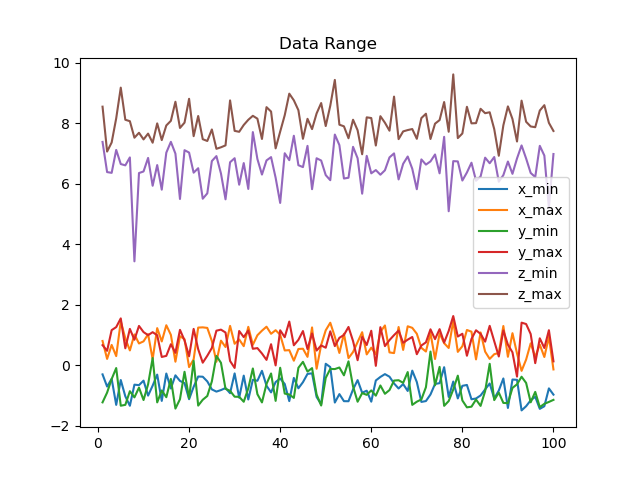
\includegraphics[width=0.45\textwidth]{./pic/Data_Extreme.png}}
	{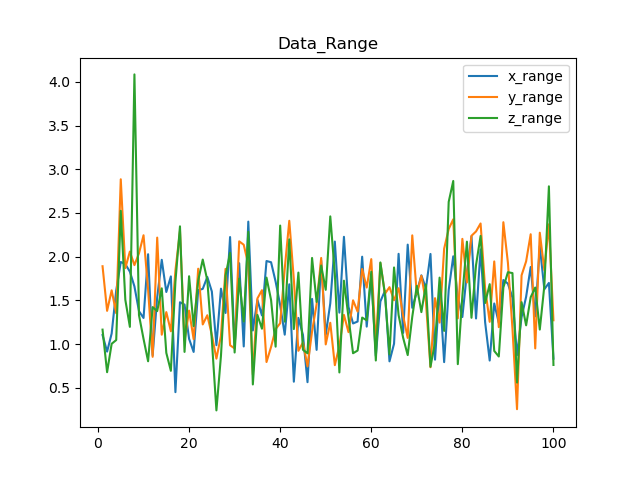
\includegraphics[width=0.45\textwidth]{./pic/Data_Range.png}}
	\label{fig:data_range}
	\caption{Left: Extreme value in 3 axis; Right: Vertex range in 3 axis}
\end{figure}

Normalize the point cloud to a unit size.

The average range and extreme value is shown in Table \ref{tab:data_range}. Choose the biggest range as a scale factor to normalize the point cloud. Use Min value to move the point clouds close to original point as much as possible.

\begin{table}[t]
	\centering
	\begin{tabular}{|c|c|c|c|}
		\hline
		Axis & Range & Min & Max\\
		\hline
		X & 1.48 & -0.75 & 0.73\\
		Y & \textbf{1.56} & -0.76 & 0.80\\
		Z & 1.47 & 6.53 & 8.00\\
		\hline
	\end{tabular}
	\caption{This is a table.}
	\label{tab:data_range}
\end{table}